\section{Stima dei parametri del sistema}
La maggior parte dei parametri possono essere misurati direttamente.
Per i parametri del motore ed il momento d'inerzia del pendolo
devo svolgere dei calcoli, che riporto in questo paragrafo.

\subsection{Momento d'inerzia del pendolo}
Il pendolo che ho usato per l'esperimento è stato realizzato con la stampa-3D,
quindi non posso calcolarne il momento d'inerzia $I$ con una semplice integrazione
(il materiale è estremamente disomogeneo all'interno).
Posso stimare $I$ conoscendo il periodo delle piccole oscillazioni $\tau_{osc}$.

L'equazione del moto, nel regime delle piccole oscillazioni, è:
\begin{align*}
    I \ddot \theta &= mgl \sin \theta \\
        &\approx mgl \theta
\end{align*}
da cui
\begin{align*}
         \omega &= \frac{2\pi}{\tau_{osc}} = \sqrt{\frac {m g l} I},\\
         \tau_{osc} &=2\pi \sqrt{\frac I {mgl}}. \numberthis\label{eq:tau-osc}
\end{align*}
La~\eqref{eq:tau-osc} permette di ricavare $I$.


\subsection{Parametri del motore}
\label{subsec:parametri-motore}
Per determinare i parametri del motore osservo il comportamento del solo
carrello quando applico un segnale $u$ costante al motore.
L'equazione che regola il comportamento del motore è la \eqref{eq:caratteristica-motore}.
L'espressione per la forza $f$
esercitata dal motore è data dalla legge di Newton
\begin{equation}
    f = M \ddot q.
    \label{eq:newton-motore}
\end{equation}
Inserisco la~\eqref{eq:newton-motore} nella~\eqref{eq:caratteristica-motore}
e applico la sostituzione
\begin{equation*}
    \left\{
    \begin{aligned}
        \dot q \mapsto v \\
        \ddot q \mapsto \dot v
    \end{aligned}
    \right.
    _.
    \label{eq:sostituzione-motore}
\end{equation*}
Ottengo
\begin{equation*}
    \dot v = \frac{u - B v} {Am}.
\end{equation*}
Fisso la condizione iniziale $v(0) = 0$ e ottengo
\begin{equation}
    v(t) = \frac u B \left(1 - e^{-\frac B {Am} t}\right).
    \label{eq:equazione-fit-motore}
\end{equation}
I parametri $A$ e $B$ sono costanti quindi, variando $u$, mi aspetto di trovare
una famiglia di curve con cui svolgere un \emph{fit} per la~\eqref{eq:equazione-fit-motore}.

Restano da modellare gli attriti.
Il carrello scorre sopra a dei cuscinetti,
quindi posso considerare l'attrito carrello-rotaia come costante.
Fa parte degli attriti anche la \emph{coppia d'impuntamento} $\tau_c$ del motore,
dovuta all'interazione tra i magneti permanenti e le armature. $\tau_c$ ha
l'andamento descritto in \autoref{fig:cogging} ed è predominante quando $\omega$ è
piccola.
Correggo entrambi gli attriti aggiungendo un offset a $u$.


%fixme i have no idea what this does but i used it so that the figure next doesn't span across
%the whole page.
%\makeatletter
%\setlength{\@fptop}{0pt}
%\makeatother

\begin{figure}[H]
    \centering
    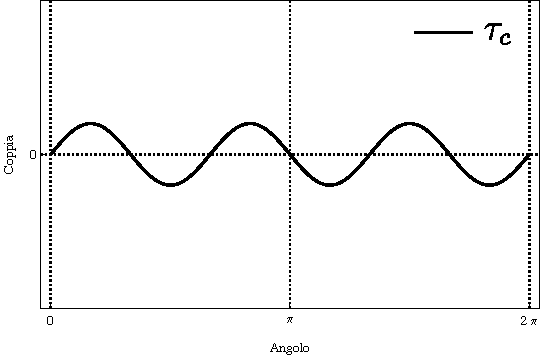
\includegraphics{assets/cogging-torque}
    \caption[Cogging torque]{Cogging toque del motore.}
    \label{fig:cogging}
\end{figure}
